% !TeX program = pdflatex
\documentclass[runningheads]{llncs}

% --- Packages ---
\usepackage[T1]{fontenc}
\usepackage[utf8]{inputenc}
\usepackage{graphicx}
\usepackage{hyperref}
\usepackage{booktabs}
\usepackage{csquotes}
\usepackage{amsmath}
\usepackage{enumitem}
\usepackage{xcolor}
\usepackage{caption}
\usepackage{subcaption}
\usepackage{tikz}
\usetikzlibrary{arrows.meta, positioning, calc}

% --- Metadata ---
\title{ThesisFlow: Plataforma Web para la Gestión y Visualización de proyectos finales y tesis en el DCIC}
\titlerunning{ThesisFlow}
\author{Ignacio Joaqu\'in Dotta}
\authorrunning{I. J. Dotta}
\institute{Departamento de Ciencias e Ingenier\'ia de la Computaci\'on (DCIC)\\
Universidad Nacional del Sur, Argentina\\
Directores: Dr. Martín Larrea y Dra. María Luján Ganuza\\
Codirector: Lic. Diego Sebastian Orbe Leiva\\
\email{\{ignacio.dotta, mlg, mll, diego.orbe\}@cs.uns.edu.ar}}

\begin{document}
\maketitle

% --- Abstract ---
\begin{abstract}
Este trabajo presenta \emph{ThesisFlow}, una plataforma web que centraliza la gestión y visualización de proyectos finales y tesis de grado del Departamento de Ciencias e Ingeniería de la Computación (DCIC). El sistema integra en una única solución los flujos administrativos de carga y curado de información, un módulo de autogestión para docentes y un portal público de analíticas interactivas. Se describen la motivación y el contexto institucional, la exploración de soluciones y alternativas, los objetivos del proyecto y los aspectos centrales de la implementación a nivel de arquitectura, modelo de datos e interfaces. Finalmente, se discuten usos concretos de la aplicación, conclusiones sobre su impacto y líneas de trabajo futuro.
\keywords{Sistemas de información académica \and Visualización de datos \and Ingeniería de software \and Aplicaciones web}
\end{abstract}

% --- 1. Motivación ---
\section{Motivación}

La gestión de proyectos finales y tesis de grado en el Departamento de Ciencias e Ingeniería de la Computación (DCIC) involucra a secretaría, docentes, estudiantes y autoridades. Históricamente, la información asociada a estos proyectos se distribuyó en planillas, documentos aislados y actas del Consejo Departamental, lo que dificulta, entre otros aspectos, mantener la trazabilidad del ciclo de vida de cada proyecto, analizar cómo evolucionan las líneas temáticas y de dirección, obtener estadísticas confiables para la planificación académica y ofrecer a los estudiantes un acceso claro y sistemático a los temas de investigación trabajados en el departamento.

\subsection*{Estado del arte}

Tradicionalmente, al preparar la producción académica anual se revisan manualmente las actas aprobadas durante el período correspondiente, obteniendo principalmente conteos agregados de proyectos finales o tesis. En años recientes se comenzó a recopilar información más detallada (título, fechas, docentes, temática, alumnos), pero sin un sistema que permita explotarla de manera estructurada ni ofrecer vistas unificadas a los distintos actores.

\subsection*{Perspectiva de los estudiantes}

Desde la óptica de los alumnos, el inicio de un proyecto final o tesis suele estar acompañado de incertidumbre. Es habitual no tener claro qué tipo de producto o alcance se espera, o contar con una idea preliminar sin saber si es viable ni qué docente podría dirigirla. A esto se suma, muchas veces, el desconocimiento sobre qué temas se han trabajado recientemente en el departamento.

Una plataforma integral que brinde acceso a proyectos históricos, sus temas y docentes asociados permite mitigar esta incertidumbre. Los estudiantes pueden explorar proyectos previos y su documentación para inspirarse, identificar tendencias temáticas a lo largo del tiempo, partir de un tema de interés y localizar qué docentes trabajan en esa área, o bien partir de un docente y reconstruir los tipos de proyectos en los que ha participado.

En este contexto, \emph{ThesisFlow} surge como una herramienta para unificar la gestión, facilitar el acceso a la información y habilitar analíticas que apoyen la toma de decisiones de estudiantes y autoridades.

% --- 2. Exploración de soluciones ---
\section{Exploración de soluciones}

Previo al diseño de la plataforma se revisaron soluciones existentes vinculadas a la gestión y difusión de proyectos finales y tesis. Entre ellas se consideraron repositorios académicos como el de la UBA (\url{https://repositoriouba.sisbi.uba.ar/gsdl/cgi-bin/library.cgi}) y el Repositorio Digital de la UNS (\url{https://repositoriodigital.uns.edu.ar/}), los cuales permiten almacenar y consultar trabajos completos, junto con metadatos básicos sobre autores, directores y fechas.

Si bien estos repositorios resultan adecuados para la difusión institucional, no incorporan flujos administrativos específicos del DCIC, como la carga a partir de actas del Consejo, ni ofrecen analíticas interactivas sobre temas, carreras o redes de colaboración. Tampoco contemplan vistas diferenciadas para secretaría, docentes y estudiantes, lo cual limita su utilidad como herramienta de gestión interna.

Además, se analizaron sistemas de gestión académica y plataformas de e-learning con módulos orientados a proyectos finales o tesis. En general, se observó que cubren parcialmente el problema y que presentan escasa capacidad de adaptación al dominio local, así como herramientas de visualización de datos poco flexibles para el tipo de análisis requerido.

% --- 3. Alternativas ---
\section{Alternativas}

A partir de la exploración previa se identificaron tres alternativas principales. La primera consistía en mantener el esquema actual, basado en planillas compartidas y documentos dispersos. Si bien esta opción requería una inversión inicial prácticamente nula, implicaba continuar conviviendo con las dificultades para garantizar la integridad y uniformidad de los datos, la escasa capacidad de visualización avanzada, la poca escalabilidad a medida que crece el volumen de proyectos y las limitaciones para extender funcionalidades o incorporar nuevos actores.

Una segunda alternativa era adoptar un sistema externo, ya sea un repositorio institucional, un sistema académico general o una plataforma de terceros. Esta opción podía reducir el esfuerzo de desarrollo, pero a costa de una menor flexibilidad para adaptar el modelo de datos al DCIC y de una fuerte dependencia de un proveedor para la evolución del sistema. Además, las capacidades analíticas y de personalización suelen estar acotadas en soluciones genéricas, lo que dificulta incorporar visualizaciones específicas o integrar los flujos administrativos existentes.

Finalmente, se consideró el desarrollo de un sistema propio, modular y extensible. Aunque esta alternativa supone un mayor esfuerzo inicial, ofrece control total sobre el modelo de datos y las reglas de negocio, permite optimizar consultas y analíticas relevantes para el departamento y habilita un diseño preparado para extenderse a nuevas carreras o módulos (por ejemplo, posgrado). Asimismo, facilita una integración progresiva con otros sistemas institucionales y consolida la soberanía sobre los datos y su explotación.

% --- 4. Especificación de objetivos ---
\section{Especificación de objetivos}

\subsection{Objetivo general}

Diseñar e implementar una plataforma web integral para la gestión, el seguimiento y la visualización de proyectos finales y tesis de grado del DCIC, que sirva como fuente confiable de información para secretaría, docentes y comunidad académica.

\subsection{Objetivos específicos}

\begin{itemize}
  \item Centralizar la información de proyectos finales y tesis en una base de datos estructurada y consistente.
  \item Proveer interfaces diferenciadas para secretaría, docentes y público general.
  \item Ofrecer analíticas interactivas sobre la producción del departamento.
  \item Incorporar mecanismos de autenticación y control de acceso acordes a cada perfil.
  \item Facilitar tareas de respaldo, restauración y auditoría de datos.
\end{itemize}

% --- 5. Implementación ---
\section{Implementación}

\subsection{Arquitectura general}

La arquitectura de \emph{ThesisFlow} adopta una estructura de tres capas: frontend, backend y base de datos. La Figura~\ref{fig:architecture} ilustra los componentes principales y sus interacciones.

\begin{figure}[h]
\centering
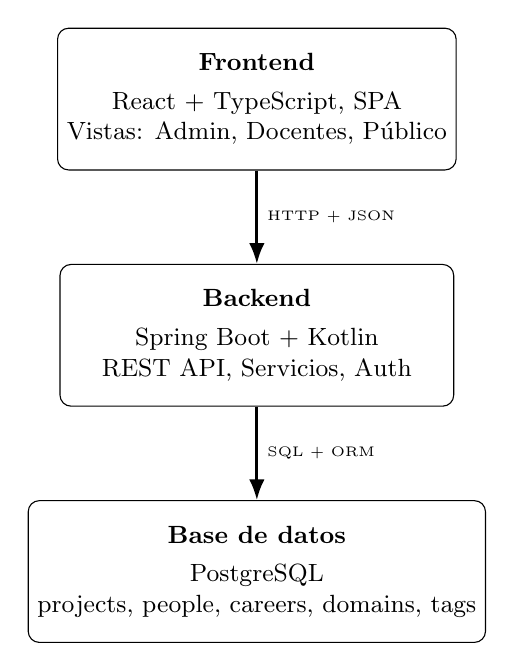
\begin{tikzpicture}[
  box/.style={
    rectangle,
    draw,
    rounded corners,
    align=center,
    minimum width=5cm,
    minimum height=1.8cm,
    font=\small
  },
  arrow/.style={-Latex, line width=1pt}
]

% Frontend (top)
\node[box] (fe) at (0, 6) {%
  \textbf{Frontend}\\[3pt]
  React + TypeScript, SPA\\
  Vistas: Admin, Docentes, Público
};

% Backend (middle)
\node[box] (be) at (0, 3) {%
  \textbf{Backend}\\[3pt]
  Spring Boot + Kotlin\\
  REST API, Servicios, Auth
};

% Base de datos (bottom)
\node[box] (db) at (0, 0) {%
  \textbf{Base de datos}\\[3pt]
  PostgreSQL\\
  projects, people, careers, domains, tags
};

% Relaciones entre capas
\draw[arrow] (fe) -- node[right, font=\tiny]{HTTP + JSON} (be);
\draw[arrow] (be) -- node[right, font=\tiny]{SQL + ORM} (db);

\end{tikzpicture}
\caption{Arquitectura general de \emph{ThesisFlow}: tres capas principales y sus responsabilidades.}
\label{fig:architecture}
\end{figure}

El backend expone endpoints REST para operaciones administrativas, vistas públicas y analíticas. Los servicios encapsulan la lógica de negocio (gestión de proyectos, personas, carreras, importación y respaldos). El frontend, implementado como SPA, organiza vistas por rol y utiliza componentes reutilizables para formularios, tablas y dashboards.

\subsection{Modelo de datos y servicios}

El modelo de datos incluye entidades como \texttt{Project}, \texttt{Person}, \texttt{Career}, \texttt{Domain} y \texttt{Tag}, junto con tablas de unión para representar relaciones muchos-a-muchos (por ejemplo, proyectos–docentes y proyectos–etiquetas). Internamente se utilizan claves enteras, mientras que hacia el exterior se exponen UUIDs para preservar estabilidad y privacidad en los identificadores.

Los servicios de negocio abstraen el acceso a datos y coordinan operaciones que involucran múltiples entidades, tales como la creación de un nuevo proyecto con sus relaciones, la importación de lotes desde archivos CSV o la construcción de agregados para analíticas.

\subsection{Decisiones de diseño y proceso de desarrollo}

El desarrollo de \emph{ThesisFlow} involucró una serie de decisiones arquitectónicas y metodológicas que respondieron tanto a los requisitos funcionales como a las necesidades operativas del DCIC.

En cuanto al mecanismo de autenticación, se optó por un esquema basado en \emph{magic links} para docentes. En lugar de gestionar usuarios y contraseñas tradicionales, el profesor solicita acceso proporcionando su correo institucional; el sistema genera un enlace único asociado a un token efímero y lo envía a esa dirección, que debe coincidir con la registrada previamente por secretaría al cargar proyectos dirigidos por ese docente. Cuando el usuario accede desde el enlace, el backend valida el token y, si es correcto, emite un JWT estándar que el frontend emplea para autenticar las sesiones posteriores. Este enfoque reduce la fricción de acceso y evita la necesidad de almacenar credenciales, apoyándose en la posesión del correo institucional como factor de autenticación.

En relación con el modelo de datos, aunque la estructura jerárquica de un proyecto final o tesis podría representarse en una base NoSQL, se decidió utilizar PostgreSQL. La elección de un esquema relacional responde a la necesidad de garantizar consistencia y normalización de datos, así como de modelar relaciones complejas entre proyectos, docentes, estudiantes, carreras y etiquetas temáticas. También facilita la realización de estadísticas precisas y agregaciones sobre datos altamente estructurados. Un enfoque NoSQL hubiera simplificado algunos aspectos del dominio, pero habría dificultado mantener la consistencia cuando cambian datos compartidos, como la información de un docente asociado a múltiples proyectos.

El proceso de desarrollo se organizó en etapas sucesivas. Primero se llevaron a cabo reuniones de análisis de requerimientos y definición del alcance general, de las cuales surgió un documento de tipo PRD (\emph{Product Requirements Document}) con los requerimientos funcionales identificados. Sobre esa base se establecieron tres grandes hitos: la construcción del modelo de datos, los CRUDs administrativos y la autenticación de secretaría; el desarrollo del acceso público, las visualizaciones interactivas y el motor de analíticas; y, por último, las funcionalidades específicas para docentes, incluyendo vistas personalizadas y el flujo de \emph{magic links}. Como apoyo al diseño de la interfaz se elaboraron maquetas en Figma, que sirvieron para validar flujos con los actores involucrados antes de avanzar en la implementación. Posteriormente se consolidó un modelo entidad–relación (ER) y se continuó con una implementación incremental, integrando componentes de backend y frontend de manera iterativa.

A lo largo del proyecto se incorporó, de manera experimental, el uso de herramientas de inteligencia artificial generativa (Claude Haiku 4.5 y Codex/ChatGPT 5.0). Estas herramientas resultaron especialmente útiles para acelerar tareas repetitivas, como la generación de componentes de frontend, código boilerplate para CRUDs, pruebas automáticas y la depuración de errores típicos de librerías. También contribuyeron en actividades de refactorización menor. En cambio, su desempeño fue más limitado en tareas complejas como el diseño del servicio de analíticas, donde tendieron a proponer soluciones conceptualmente incorrectas o poco eficientes. En síntesis, la experiencia sugiere que la IA puede reducir de manera significativa los tiempos de desarrollo en proyectos de escala media cuando se aplica a problemas bien acotados y se la utiliza bajo supervisión humana.

\subsection{Despliegue e infraestructura}

En el entorno actual, el frontend de \emph{ThesisFlow} se despliega en Vercel, que realiza el proceso de construcción utilizando la configuración de Vite.js y sirve los archivos estáticos resultantes desde su red de distribución de contenido. El backend y la base de datos PostgreSQL se alojan en Render, donde el servicio backend se construye y ejecuta a partir de un \texttt{Dockerfile}, lo que permite reproducir localmente el mismo entorno de ejecución que en producción.

Como línea de mejora, se considera deseable que a futuro la plataforma sea alojada en la infraestructura del propio DCIC, bajo un dominio institucional del tipo \texttt{*.cs.uns.edu.ar}, de modo de consolidar el control operativo, la soberanía de los datos y la integración con otros servicios de la Universidad.

\subsection{Carga inicial de datos}

La carga inicial de datos constituyó una etapa fundamental para poner en funcionamiento la plataforma con un conjunto completo y confiable de proyectos finales y tesis históricos. El proceso se estructuró en tres fases principales: normalización del dataset original, preparación estructurada de los archivos y carga mediante la funcionalidad de importación masiva del sistema.

\paragraph{Normalización y limpieza del dataset.}
El punto de partida fue un conjunto heterogéneo de fuentes: planillas históricas, documentos administrativos y actas del Consejo Departamental. Estos datos presentaban variaciones en nombres de docentes, formatos de fechas, diferencias tipográficas y estructuras inconsistentes.  
Para unificar estos registros, se desarrolló un script específico (documentado en el repositorio del proyecto) que se encargó de estandarizar nombres de docentes y estudiantes mediante reglas de coincidencia aproximada y diccionarios de equivalencias, unificar los distintos formatos de fechas (aprobación, defensa, publicación), asignar carreras y dominios respetando las taxonomías actuales del DCIC, detectar y resolver duplicados a partir de heurísticas basadas en combinaciones de título, año y docente, y generar identificadores UUID estables para cada proyecto y cada persona. Este proceso garantizó un dataset coherente y apto para ser cargado en un modelo relacional.

\paragraph{Preparación del archivo de importación.}
Una vez normalizado el dataset, el script generó un archivo CSV con columnas alineadas al modelo de datos interno: proyecto, fechas, docentes, carrera, etiquetas temáticas y dominios.  
El sistema comprueba automáticamente la validez del archivo, la consistencia de las columnas y el tipo de datos antes de continuar.

\paragraph{Importación masiva en la plataforma.}
Finalmente, la carga se realizó utilizando la funcionalidad de “Importar proyectos”, que:

\begin{itemize}
  \item procesa cada fila como una operación atómica (validación → creación del proyecto → creación de relaciones);
  \item informa errores fila por fila sin detener el proceso completo;
  \item genera un reporte detallado con estadísticas (creados, actualizados, rechazados);
  \item asegura que las entidades relacionadas (docentes, etiquetas, dominios) se creen o reutilicen según corresponda.
\end{itemize}

Gracias a este proceso, el sistema quedó poblado con la totalidad del historial disponible, permitiendo que las visualizaciones y analíticas fueran significativas desde el primer despliegue.

\subsection{Flujo de creación de proyectos}

El flujo de creación de un proyecto refleja el proceso que sigue la secretaría para registrar un proyecto final o tesis aprobado. La Figura~\ref{fig:sequence} muestra un diagrama de secuencia simplificado.

\begin{figure}[h]
\centering
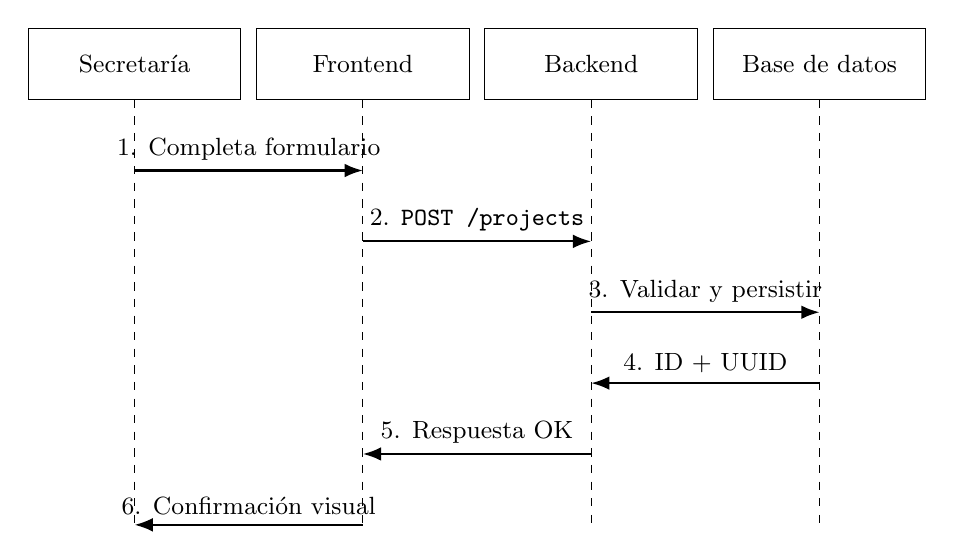
\begin{tikzpicture}[
  font=\small,
  lifeline/.style={rectangle, draw, minimum width=2.7cm, minimum height=0.9cm, align=center},
  flow/.style={-Latex, line width=0.8pt},
  x=2.9cm,
  y=1cm
]

% Lifeline headers
\node[lifeline] (admin) at (0,0) {Secretaría};
\node[lifeline] (fe) at (1,0) {Frontend};
\node[lifeline] (be) at (2,0) {Backend};
\node[lifeline] (dbs) at (3,0) {Base de datos};

% Lifeline dashed
\draw[dashed] (admin.south) -- ++(0,-5.4);
\draw[dashed] (fe.south) -- ++(0,-5.4);
\draw[dashed] (be.south) -- ++(0,-5.4);
\draw[dashed] (dbs.south) -- ++(0,-5.4);

% Messages (explicit vertical levels)
\draw[flow] ($(admin.south)+(0,-0.9)$) -- node[above]{1. Completa formulario} ($(fe.south)+(0,-0.9)$);
\draw[flow] ($(fe.south)+(0,-1.8)$) -- node[above]{2. \texttt{POST /projects}} ($(be.south)+(0,-1.8)$);
\draw[flow] ($(be.south)+(0,-2.7)$) -- node[above]{3. Validar y persistir} ($(dbs.south)+(0,-2.7)$);
\draw[flow] ($(dbs.south)+(0,-3.6)$) -- node[above]{4. ID + UUID} ($(be.south)+(0,-3.6)$);
\draw[flow] ($(be.south)+(0,-4.5)$) -- node[above]{5. Respuesta OK} ($(fe.south)+(0,-4.5)$);
\draw[flow] ($(fe.south)+(0,-5.4)$) -- node[above]{6. Confirmación visual} ($(admin.south)+(0,-5.4)$);

\end{tikzpicture}

 \caption{Flujo simplificado de creación de un proyecto en \emph{ThesisFlow}.}
 \label{fig:sequence}
\end{figure}

Este flujo asegura que los datos ingresados se validen en el backend, que se creen las relaciones necesarias en la base de datos y que el nuevo proyecto quede disponible inmediatamente para las interfaces de consulta y analíticas.

\begin{figure}[h]
\centering
\fbox{\parbox{0.8\linewidth}{Espacio reservado para una captura de pantalla del panel de administración de proyectos en \emph{ThesisFlow}.}}
\caption{Vista de administración de proyectos (captura de pantalla a incorporar).}
\label{fig:admin-screenshot}
\end{figure}

% --- 6. Usos de la app ---
 \section{Usos de la aplicación}

\emph{ThesisFlow} se utiliza en distintos escenarios por actores con necesidades diversas. Desde la secretaría, la plataforma funciona como herramienta central para registrar proyectos finales o tesis aprobados, actualizar metadatos y generar listados consolidados. Los docentes la emplean para consultar los proyectos en los que participan como directores o co-directores y verificar la información publicada sobre su actividad de dirección. Finalmente, el público general puede explorar la producción del departamento mediante filtros y visualizaciones interactivas que ponen en contexto la trayectoria académica del DCIC.

\subsection*{Ejemplo de uso por secretaría}

Un caso típico de uso por parte de la secretaría se da cuando el Consejo Departamental aprueba un nuevo proyecto final o tesis. El personal administrativo inicia sesión en el módulo de administración y accede al panel principal, desde donde puede navegar al catálogo de proyectos. Allí inicia el asistente de creación de proyecto, que guía el ingreso de la información básica: título, tipo de trabajo, carrera, resumen y fechas relevantes. En una segunda etapa del asistente se seleccionan los directores y co-directores a partir del catálogo de docentes ya cargado en el sistema, mientras que en una tercera etapa se incorporan los estudiantes involucrados, ya sea seleccionándolos del listado existente o ingresándolos manualmente según la información disponible.

Al confirmar la operación, el sistema valida los datos, crea el nuevo registro de proyecto y establece las relaciones con docentes, estudiantes, carrera y dominios de aplicación. De este modo, el proyecto queda inmediatamente incorporado al registro histórico, disponible tanto para las visualizaciones públicas como para las consultas internas. Cuando se trata de actualizar grandes volúmenes de información (por ejemplo, al incorporar varios años de proyectos históricos), la secretaría puede utilizar en cambio la funcionalidad de importación masiva a partir de archivos CSV normalizados, lo que reduce errores y agiliza la carga inicial o las actualizaciones periódicas.

\subsection*{Ejemplo de uso por docentes}

Desde la perspectiva de los docentes, la plataforma ofrece un punto de acceso unificado para revisar y completar la información asociada a los proyectos en los que participan. El flujo comienza cuando el profesor solicita un enlace de acceso desde la página pública de \emph{ThesisFlow}, ingresando su correo institucional. El sistema genera un \emph{magic link} temporal y lo envía por correo electrónico; al hacer clic en el enlace, se valida el token y se emite un JWT que permite acceder al panel de docente sin necesidad de gestionar contraseñas.

Una vez en el panel, el docente visualiza un listado de proyectos filtrado automáticamente según su rol de director o co-director. Desde allí puede acceder al detalle de cada proyecto para revisar el título, la descripción, los estudiantes asociados, la carrera, el dominio de aplicación y las etiquetas temáticas. Cuando un proyecto ha concluido, el docente puede completar o ajustar los metadatos finales, incorporando la fecha de finalización, la calificación, palabras clave adicionales y la selección definitiva de etiquetas y dominios. En aquellos casos en que la política institucional lo permita, también puede asociar un enlace o recurso con la memoria del trabajo. Además, el docente cuenta con vistas de analíticas que reutilizan los mismos datos públicos, pero filtradas por su propia actividad de dirección, lo que le permite seguir la evolución de sus líneas de trabajo a lo largo del tiempo.

\subsection*{Ejemplo de uso por estudiantes}

Un estudiante próximo a iniciar su proyecto final o tesis accede a la sección pública de \emph{ThesisFlow} sin necesidad de autenticación. Desde la vista de catálogo puede navegar por un listado paginado de proyectos históricos y aplicar filtros por carrera, dominio de aplicación, etiquetas temáticas, docentes o año de finalización. Esta combinación de filtros le permite acotar rápidamente el conjunto de proyectos a aquellos que se aproximan a sus intereses, por ejemplo, trabajos recientes de su carrera en temas de sistemas distribuidos o aprendizaje automático.

Al seleccionar un proyecto en el catálogo, el sistema muestra una vista detallada con el título, la descripción, los docentes responsables, la carrera, el dominio y las etiquetas temáticas asociadas. A partir de esta información, el estudiante puede identificar patrones sobre el tipo de problemas abordados, el nivel de complejidad esperado y los recursos típicos empleados. Complementariamente, el estudiante puede recorrer el portal de analíticas públicas, que incluye líneas de tiempo, mapas de calor de temas y redes de colaboración entre docentes, para comprender mejor cómo se distribuyen los proyectos por año, tópico y dirección. En conjunto, estas vistas sirven como insumo para formular una propuesta propia más informada y ubicar potenciales directores afines a sus intereses.

% --- 7. Conclusiones ---
% --- 7. Conclusiones y trabajo futuro ---
\section{Conclusiones y trabajo futuro}

El desarrollo de \emph{ThesisFlow} dotó al DCIC de una herramienta específica para la gestión y visualización de proyectos finales o tesis de grado. La plataforma permitió reducir la fragmentación de la información y la dependencia de planillas dispersas, mejorar la accesibilidad de los datos académicos y habilitar nuevas formas de análisis sobre la producción del departamento. Desde la perspectiva de ingeniería de software, el sistema constituye un caso de estudio de diseño e implementación de una aplicación web modular, con separación clara de responsabilidades, API REST y componentes de visualización de datos aplicados a un problema académico real.

La experiencia de desarrollo también dejó varias lecciones. La decisión de utilizar un modelo relacional y un motor de analíticas en memoria resultó adecuada para la escala actual de datos, aunque deja abierta la necesidad de optimizar consultas y explorar mecanismos de caching o vistas materializadas en escenarios de mayor volumen. Del mismo modo, la incorporación de mecanismos de autenticación basados en \emph{magic links} facilitó el acceso de los docentes sin agregar complejidad a la gestión de credenciales.

En cuanto al trabajo futuro, se identifican varias líneas de evolución. En el plano técnico, resulta natural avanzar hacia la optimización de las analíticas mediante caching y/o almacenamiento auxiliar de resultados preprocesados, así como extender la cobertura a proyectos de posgrado y eventualmente a otros departamentos de la Universidad. También se considera relevante integrar la plataforma con sistemas institucionales existentes (como los sistemas de gestión académica o los repositorios digitales) y fortalecer los mecanismos de auditoría y trazabilidad de cambios.

Desde el punto de vista funcional, una línea de desarrollo interesante es permitir que los propios alumnos suban recursos asociados a sus trabajos (código, datasets, documentación complementaria) y mejorar el soporte de almacenamiento de archivos dentro del sistema, reduciendo la dependencia de enlaces externos. Finalmente, la incorporación de estrategias de respaldo automático y procedimientos simplificados de restauración contribuirá a robustecer el sistema como componente permanente de la infraestructura académica del DCIC.

\subsubsection*{Agradecimientos}
Agradezco especialmente a mis directores, Dr. Martín Larrea y Dra. María Luján Ganuza, y a mi codirector, Lic. Diego Sebastián Orbe Leiva, por su guía, dedicación y acompañamiento durante el desarrollo de este trabajo. Su orientación académica y técnica fue fundamental para la concreción de este proyecto.

% --- Bibliografía ---
\bibliographystyle{splncs04}
\bibliography{references}

\end{document}
